\section{Lineare Zeitinvariante System (LTI)}
\subsection{Laplace-Transformation}


 	\subsubsection{Eigenschaften}
  		\renewcommand{\arraystretch}{2}
		\begin{tabularx}{\textwidth}{|l|X|}
        	\hline
        	Linearität & 
 			$a\cdot f(t) + \beta\cdot g(t) \laplace a\cdot F(s) + \beta\cdot
 			G(s)$ \\
 			\hline
 			"Ahnlichkeit / Streckung &
 			$f(a t) \laplace \frac{1}{a}F \left (\frac{s}{a} \right ) \quad 0
 			<a \in\mathbb{R}$ \\
 			\hline
 			Faltung im Zeitbereich &
 			$f(t) \ast g(t) = \int\limits_{0}^{t} f(\tau)g(t-\tau)d\tau \laplace F(s)
 			\cdot G(s)$\\
 			\hline
 			Faltung im Frequenzbereich &
 			$f(t) \cdot g(t) \laplace \frac{1}{2\pi j}\int\limits_{c-j\infty}^{c+j\infty}
 			F(\xi) G(s-\xi)d\xi$ \\
 			\hline
 			Ableitung im Zeitbereich &
 			$\frac{\partial f(t)}{\partial t} \laplace sF(s)
 			-f(0^+)$ \\
 			\hline
 			Ableitungen im Zeitbereich &
 			$\frac{\partial^n f(t)}{\partial t^n} \laplace s^nF(s)
 			-s^{n-1}f(0^+)-s^{n-2}\frac{\partial f(0^+)}{\partial t}-\ldots
 			-s^0\frac{\partial^{n-1} f(0^+)}{\partial t^{n-1}}$ \\
 			\hline
 			Multiplikation mit $t$ &
 			$t\cdot f(t)  \laplace \frac{-\partial F(s)}{\partial s}$ \\
 			\hline
 			Ableitung im Frequenzbereich &
 			$(-t)^n f(t) \laplace  \frac{\partial^n F(s)}{\partial s^n}$ \\
 			\hline
 			Verschiebung im Zeitbereich nach rechts &
 			$f(t - t_0) \laplace F(s)e^{- t_0 s}$ \\
 			\hline
			Verschiebung im Zeitbereich nach links &
			$f(t + t_0) \laplace e^{t_0 s} \cdot [F(s) - \int\limits_0^{t_0} f(t) \cdot e^{-st} dt]$\\
			\hline
 			Verschiebung im Frequenzbereich (Dämpfungssatz) &
 			$f(t)e^{\mp a t} \laplace F(s\pm a)$ \\
 			\hline
 			Integration &
 			$\int\limits_0^t f(\tau)d\tau \laplace \frac{1}{s}F(s)$ \\
 			\hline
 			Anfangswerttheorem &
 			$\lim_{t\rightarrow 0^+} f(t) = \lim_{s\rightarrow \infty} s \cdot F(s),\text{~wenn
 			}  \lim_{t\rightarrow 0} f(t)\text{~existiert}.$ \\
 			\hline
 			Endwerttheorem &
 			$\lim_{t\rightarrow \infty} f(t) = \lim_{s\rightarrow 0} s \cdot F(s),\text{~wenn
 			}  \lim_{t\rightarrow \infty} f(t)\text{~existiert.}$ \\
 			\hline
       	\end{tabularx}
\newpage
	\subsection{Laplace-Tabelle}
	\begin{multicols}{2}
		\begin{center}
			\begin{tabular}{|lcc|}
				\hline
				$\delta \left( t \right)$ & $\laplace$ & $1$ \\
				$\delta \left( t - a \right)$ & $\laplace$ & $e^{- a s}$\\
				$\sigma \left( t \right)$ = $\varepsilon \left( t \right)$ & $\laplace$ & $\frac{1}{s}$ \\
				$\sigma \left( t \right) \cdot t$ & $\laplace$ & $\frac{1}{s^2}$\\
				$\sigma \left( t \right) \cdot t^2$ & $\laplace$ & $\frac{2}{s^3}$\\
				$\sigma \left( t \right) \cdot t^n$ & $\laplace$ & $\frac{n!}{s^{n+1}}$\\
				$\sigma \left( t \right) \cdot e^{a t}$ & $\laplace$ &
				$\frac{1}{s-a}$\\
				$\sigma \left( t \right) \cdot t \cdot e^{a t}$ & $\laplace$ &
				$\frac{1}{( s - a )^2}$\\
				$\sigma \left( t \right)\cdot t^2 \cdot e^{a t}$ &
				$\laplace$ & $\frac{2}{{( s - a )}^3}$\\
				$\sigma \left( t \right)\cdot t^n \cdot e^{ a t}$ &
				$\laplace$ & $\frac{n!}{(s-a)^{n+1}}$\\
				$\sigma \left( t \right) \cdot (1-e^{a t}$) & $\laplace$ &
				$\frac{- a}{s ( s - a )}$\\
				$\sigma \left( t \right) \cdot \cos \left(b t \right)$ & $\laplace$ &
				$\frac{s}{ s^2 + b^2}$\\
				$\sigma \left( t \right) \cdot \sin \left(b t \right)$ & $\laplace$ &
				$\frac{b}{s^2 + {b^2}}$\\
				$\sigma \left( t \right) \cdot e^{a t} \cdot \cos \left(b t \right)$ & $\laplace$ &
				$\frac{s- a}{ (s- a)^2 + b^2}$\\
				$\sigma \left( t \right) \cdot e^{a t} \cdot \sin \left(b t \right)$ & $\laplace$ &
				$\frac{b}{(s- a)^2 + {b^2}}$\\
				$\sigma \left( t \right) \cdot \frac{e^{a t} - e^{b t}}{a-b}$ & $\laplace$ & $\frac{1}{(s-a)(s-b)}$ \\
				$\sigma \left( t \right) \cdot \frac{a e^{a t} - b e^{b t}}{a-b}$ & $\laplace$ & $\frac{s}{(s-a)(s-b)}$\\
				\hline
			\end{tabular}
		\end{center}
	\columnbreak
		\begin{center}
	\[\boxed{F(s)=\int\limits_0^\infty f(t)e^{-st}dt} \qquad s=\sigma+j\omega\]\\
\subsubsection{Bedingungen}
\begin{itemize}
		\item Definitionsbereich nur für kausale Systeme $t\geq 0$\\
		\item Integrierbar über das Intervall $(0,\infty)$\\
		\item Wachstum kleiner als der von eienr Exponentialfunktion\\ 
		\item Gegen"uber $j\omega$ bei der Fourier-Transformation ist bei der
			Laplace-Transformation $s$ verallgemeinert zu $s=\sigma + j\omega$. Das
			bedeutet, dass die Fourier-Transformierte $F(j\omega)$ durch die
			Laplace-Transformation $F(s)$ ausgedr\"uckt werden kann. \\
		\item mit $\sigma = 0 \rightarrow$ Amplitude bleibt konstant\\
		\item mit $\sigma > 0 \rightarrow$ explodiert die Amplitude f\"ur $0 < t \rightarrow \infty$ \\
		\item mit $\sigma < 0 \rightarrow$ klingt die Amplidute für $0 < t \rightarrow \infty$ auf $0$ ab
\end{itemize}

	\subsubsection{Vorgehen Rücktransformation}
		\begin{enumerate}
			\item Kürzen oder vereinfachen
			\item Rücktransformation mittels Laplace-Tabelle
			\item Partialbruchzerlegung falls nötig
			\item $h(t)\hspace{0.2cm}\underline{nicht} < 0$
		\end{enumerate}
	\end{center}
\end{multicols}

\subsection{Differentialgleichungen lösen}
Die ‘interne’ Beschreibung transformieren, fallen Probleme mit Anfangsbedingungen weg, da man näher
an den physikalischen Grössen bleibt
\begin{multicols}{2}
		\begin{center}
			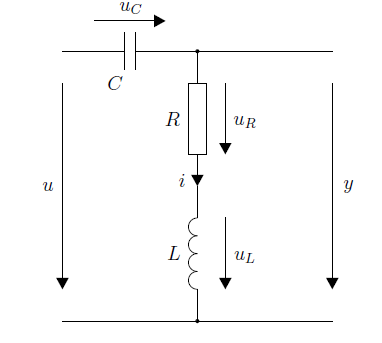
\includegraphics[width=6cm]{./images/diffgleichung.png}
		\end{center}
	\columnbreak
\begin{center}
	\begin{tabular}{ll}
		$i(t) = C \cdot \dot{u}_{C}(t)$ & Kapazität  \\
		$uL(t) = L \cdot \dot{i}(t)$ & Induktivität \\
		$uR(t) = R \cdot i(t)$ & Widerstand \\
		$u(t) = u_{C}(t) + u_{R}(t) + u_{L}(t)$ & Maschengleichung, links \\
		$y(t) = u_{R}(t) + u_{L}(t)$ & Maschengleichung, rechts \\
	\end{tabular}
\end{center}
\end{multicols}

\begin{multicols}{2}
{	$I(s) = C  \cdot  [s  \cdot  U_{C}(s) - u_{C}(0)]$ \\
	$U_{L}(s) = L  \cdot  [s  \cdot  I(s) - i(0)]$ \\
	$U_{R}(s) = R  \cdot  I(s)$ \\
	$U(s) = U_{C}(s) + U_{R}(s) + U_{L}(s)$ \\
	$Y (s) = U_{R}(s) + U_{L}(s)$ \\}

	\columnbreak
\begin{center}

$Y(s) = \frac{s^2 LC+sRC}{s^2 LC +sRC +1}\cdot U(s) + \frac{[sLC + RC] \cdot u_{C}(0) + L \cdot i(0)}{s^2 LC +sRC +1}$
\end{center}
\end{multicols}

Auch hier beinhaltet das Gleichungssystem 5 Gleichungen und 6 Signale. Das Eliminieren der 4 internen Signale $(U_{C}, U_{R}, U_{L}, I)$ fällt hier leichter. Offensichtlich sind hier weniger Anfangsbedingungen nötig als wenn nur eine Gleichung in den Bildbereich transformiert wird.

\subsection{Übertragungsfunktion UTF}
\hspace{2.3cm}G(s)\\
$Y(s) = \underbrace{\frac{\overbrace{s^2 LC+sRC}}{s^2 LC +sRC +1}\cdot U(s)} + \underbrace{\frac{[sLC + RC] \cdot u_{C}(0) + L \cdot i(0)}{s^2 LC +sRC +1}}$ \newline
\textcolor{white}{x} \hspace{2.4cm} $Y_{E}(s)$ \hspace{3.8cm} $Y_{F}(s)$ \\
Das Ausgangssignal Y (s) setzt sich aus den beiden Termen $Y_{E}(s) und Y_{F}(s)$ zusammen.Der erzwungene Anteil $Y_{E}(s)$ ist durch das Eingangssignal U(s) bestimmt, aber unabhängig von den Anfangsbedingungen des Netzwerks.
Beim freien Anteil $Y_{F}(s)$ ist es umgekehrt; dieser hängt nur von den Anfangsbedingungen,
nicht aber vom Eingangssignal ab. Die freie Antwort zeigt also, wie
das System sich verhält, wenn man es ‘sich selbst überlässt’
$\text{für} u_{C}(0) \neq 0 \text{ und } \diagup \text{ oder } i_{L}(0) \neq 0$
\begin{itemize}
	\item $ y_{F}(t) die Form y_{F,1} \cdot e^{\lambda_{1}t} + y_{F,2} \cdot e^{\lambda_{1}t} \text{ haben muss, wobei}$
	\item $ \lambda_{1,2}= \frac{-RC \pm \sqrt{(RC)^2 - 4 \cdot LC} }{2 \cdot LC}$ die Wurzeln des charakteristischen Polynoms sind,
	\item und die Werte $y_{F,1} \text{ und } y_{F,2}$ sich aus den Anfangsbedingungen ergeben.
\end{itemize}